
The scoring function, as mentioned in ~\ref{inlining:scoring} estimates the
fitness of a function to be inlined, this way a function whose score is above
zero ($0$) may be inlined, if the budget allows. But the algorithm that decides
which function will be inlined is solely based in this information, not in the
current budget value, nor in the other scores computed.

In \cite{BerubePhD} the inlining algorithm sorts the candidates for inlining
based on the score function. As the score takes into account estimated values for
benefit and cost of inlining, we suggest to use it but aggregating the expenditure,
the budget, and other scores besides the most fitted.

The idea is to perform a more compĺete version of the knapsack algorithm considering
all the scores above zero and the budget (the ``size'' of the knapsack). Proceeding
this way we can optimize the amount of budget wasted for inlining.

To make sure that there is some room for improvement in the choice of the next
function to be inlined, we are comparing the original choice (just using the highest
score) with two different ways of choosing, a random choice, and the ``more complete''
knapsack choice. Our experiments have shown that there is a best way of choosing the
candidates for the inliner, table \refTable{tab:choice} shows the results for these
three algorithms.\rr{table \refTable{tab:choice} is dummy}

\begin{table}
  \centering
  \begin{tiny}
  
\begin{tabular}{lllll}

{\bf T} & {\bf C} & {\bf Quantiles (\%)} & 
  {\bf Description} & {\bf Evaluation Name} \\ \hline

P & -- & 25 & first quartile   & QPointQ=25 \\
P & -- & 50 & estimated median & QPointQ=50 \\
P & -- & 75 & third quartile   & QPointQ=75 \\

P & L & 50, 75 & average and optimistic      & QPLinearQ=50,75 \\
P & NL   & 50, 75 &                             & QPSqrtQ=50,75   \\
P & L & 5, 95  & worst and best w/o outliers & QPLinearQ=5,95  \\
P & NL   & 5, 95  &                             & QPSqrtQ=5,95    \\

R & -- & \pair{50}{100} & top half: optimistic & QRangeQ=50,100 \\
R & -- & \pair{25}{75}  & ``central'' average  & QRangeQ=25,75  \\
R & -- & \pair{5}{95}   & average w/o outliers & QRangeQ=5,95   \\

R & L & \pair{0}{25}, \pair{75}{100} & pessimistic and optimistic
  & QRLinearQ=0,25,75,100 \\
R & NL   & \pair{0}{25}, \pair{75}{100} & 
  & QRSqrtQ=0,25,75,100 \\

\hline
\end{tabular}

  \end{tiny}
  \caption{Running time of experiments, considering $3$-times run}
  \label{tab:choice}
\end{table}

The results shown in figure \refFigure{fig:choice} refer to the geometric mean of all
the runs for each program and each input data. We have the running time for each program
in the $y$-axis, and the programs and input data on the $x$-axis. The performance of the
three different algorithms are shown for comparison.\rr{figure \refFigure{fig:choice} is dummy}

\begin{figure}
  \centering
  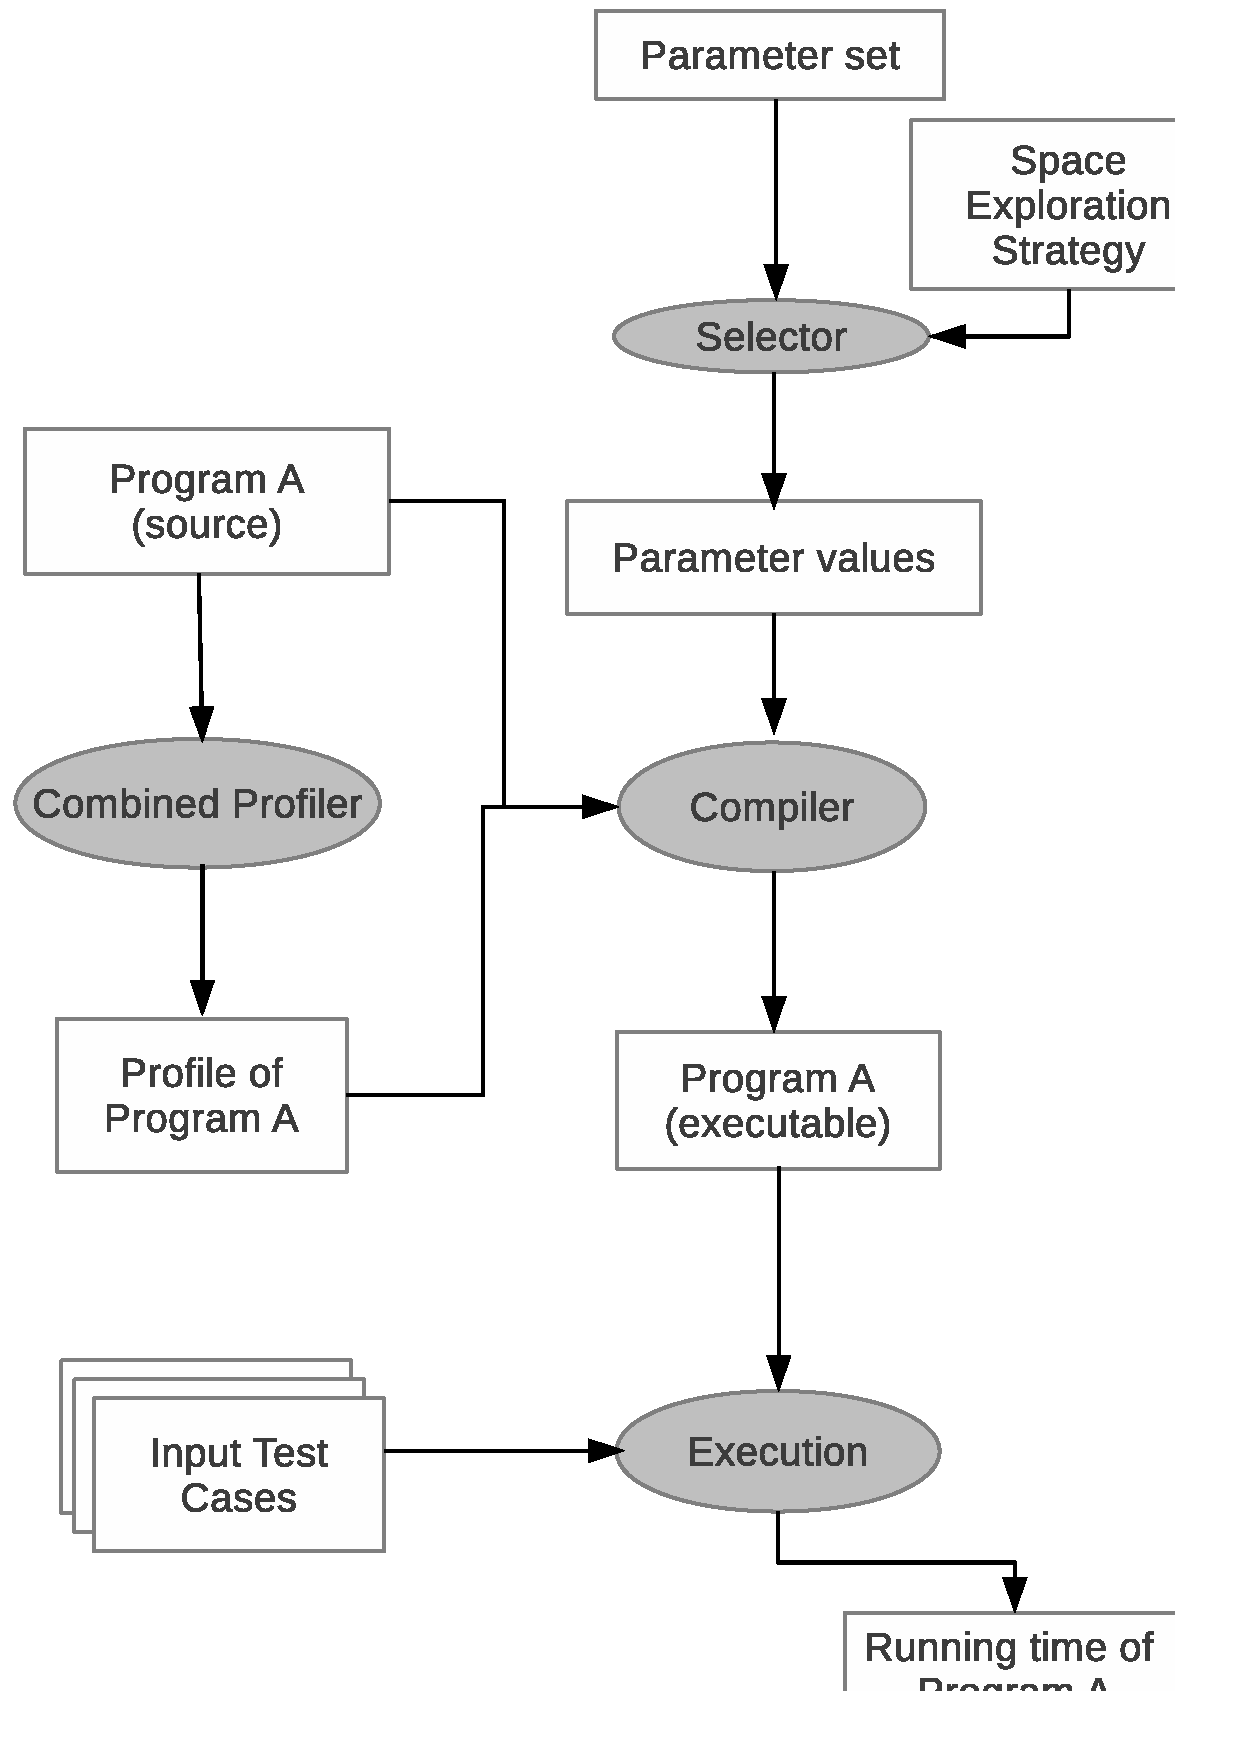
\includegraphics[width=0.50\linewidth]{Figures/choice}
  \caption{Algorithms for choosing the candidates}
  \label{fig:choice}
\end{figure}
